La fluidodinamica computazionale, spesso abbreviata con CFD, è un metodo per risolvere e analizzare problemi di fluidodinamica attraverso l'analisi numerica su calcolatore.
Viene utilizzata specialmente nel campo dell'industria e della ricerca per tutto ciò che concerne problematiche che riguardano l'interazioni di fluidi con altre superfici all'interno di un dominio.
Alla base del funzionamento di tutti i software di CFD risiede la capacità di risolvere le equazioni di Navier-Stokes (\ref{navierstokes}) congiuntamente alle equazioni ad esse collegate.
Come anticipato nel Capitolo \ref{cap:capitoli/capitolo2/capitolo2} la soluzione esatta a questi problemi accade solo in presenza di semplici flussi laminari che interagiscono con geometrie semplici,
la maggior parte dei casi ovviamente non ricade in questi casi e risultano quindi necessari degli approcci approsimati attraverso metodi numerici.

Analizziamo di seguito i passi necessari per portare a termine una generica simulazione fluidodinamica, definiti in base all'ordine con cui vengono eseguiti solitamente.
\section{Modello 3D}
Un modello tridimensionale, o 3D, è la rappresentazione di un oggetto tridimensionale basata su notazione matematica. Risiede alla base di ogni simulazione CFD poiché rappresenta l'oggetto con cui
il fluido da simulare interagirà. A seconda delle necessità legate alla simulazione è possibile realizzare modelli di superifici ideali (superfici in tre dimensioni ma con spessore infinitamente piccolo), anche chiamati
Boundary-based objects, o di oggetti solidi che occupano un volume, detti Volume-based objects, spesso costruiti attraverso forme geometriche lementari.
Gli oggetti basati su volumi sono quelli più usati in ambito CFD perché rappresentano un vero e proprio corpo con proprietà fisiche reali (massa, volume, centro di gravità, momenti, densità).
Proprio grazie a queste proprietà possiamo influenzare le simulazioni CFD. Il modello 3D di ciò che si sta simulando può essere considerato come il "negativo" della mesh, ovvero l'oggetto da
cui viene discretizzato il volume e creata la relativa mesh.
\section{Discretizzazione del volume}
Uno dei processi più delicati delle simulazioni CFD è proprio quello della discretizzazione del dominio di interesse. Discretizzare significa trasformare modelli matematici ed equazioni continue
in entità discrete, ed è alla base di ogni tipo di computazione matematica effettuata da un calcolatore. Nel caso della discretizzazione di un volume si tenta di trasformare una regione di spazio
continuo tridimensionale in un oggetto comprensibile dal calcolatore, spesso si tratta di un oggetto composto da punti dotati di tre dimensioni che formano delle geometrie tridimensionali.
Intrinsecamente a ogni discretizzazione vi è una inevitabile perdita d'informazione, minore questa perdita e maggiore sarà la risoluzione della simulazione.

    \subsection{Mesh}\label{mesh}
    Il processo che discretizza un dominio è chiamato anche generazione di mesh che non è altro che l'insieme di tutti gli elementi utilizzati per discretizzare lo stesso.
    In termini pratici una mesh è un reticolo di punti che definiscono un oggetto, composto da vertici, spigoli e facce.
    La mesh è composta da geometrie semplici primitive definite matematicamente (detti anche elementi finiti), principalmente si tratta di triangoli o quadrilateri per i domini bidimensionali e
    di esaedri e tetraedri per quelli tridimensionali. Naturalmente per modellare particolari curve, o in generale elementi complessi, è possibile avvalersi di diverse geometrie primitive.
    Una volta creata una mesh è possibile aumentarne la risoluzione attraverso processi di suddivisione che rendono più accurati i risultati generati, incrementando significatamente i tempi di simulazione.
    \begin{figure}[H]
        \centering
        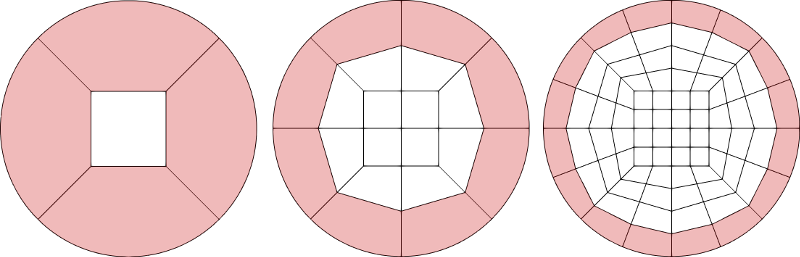
\includegraphics[width=\linewidth]{figure/subdivision.png}
        \caption{Esempio di mesh bidimensionali e relative suddivisioni.}
    \end{figure}

\section{Solver}\label{solver}
Nei capitoli precedenti abbiamo descritto i problemi la cui risoluzione è necessaria per computare correttamente le simulazioni fluidodinamiche, in questa sezione analizziamo come agiscono i
solutori (Solver) per trovare correttamente e nel minor tempo possibile tali soluzioni.
Un solver non è altro che un qualsiasi programma, o parte di programma, che dati in input:
\begin{itemize}
    \item Mesh
    \item Equazioni Navier-Stokes
    \item Condizioni al contorno
    \item Costanti fisiche
    \item Parametri di discretizzazione temporale
\end{itemize}
riesce a computare una soluzione accettabile e produrre in output una serie di risultati comprensibili da programmi di visualizzazione o post processing.
Nelle sottosezioni seguenti analizzeremo nel dettaglio alcuni importanti concetti relativi al solutore argomento di questa tesi.

    \subsection{Condizioni al contorno}\label{boundary_conditions}
    Le condizioni iniziali e al contorno sono necessarie a definire correttamente il problema che si sta cercando di risolvere. Rappresentano parametri di cui conosciamo il comportamento durante il tempo
    e che possiamo inserire all'interno delle nostre equazioni di Navier-Stokes per tentare di risolvere il sistema.
    Esempi di condizione al contorno, contestualizzati con il caso in esame,  possono essere la velocità di ingresso del flusso all'interno dell'ugello, la temperatura iniziale del flusso,
    la pressione iniziale del flusso, il volume irradiato dal fascio laser. Altri tipi di condizioni al contorno molto importanti per lo sviluppo di questo progetto sono tutte la definizione
    di tutte le superfici che si comportano come ostacolo per il flusso e le particelle, comunemente chiamati wall (muri). I wall di solito vengono definiti per mezzo di ulteriori parametri quali:
    rugosità, spessore, temperatura, ecc...

    \subsection{Interpolazione}\label{interpolazione}
    Per interpolazione si intende il processo atto a individuare, a partire da un insieme finito di punti, nuovi punti all'interno di un sistema di coordinate attraverso delle funzioni.
    Nelle simulazioni CFD la fase di interpolazione è critica in quanto è quella che effettivamente calcola, per ogni grado di libertà della simulazione, la soluzione delle funzioni associate calcolate
    nel determinato punto.
    La figura \ref*{fig:interpolazione} rappresenta un esempio di interpolazione su mesh di punti tridimensionali, notare lo spostamento degli stessi tra il frame iniziale, indicato tramite \textit{wireframe} e quello finale
    . Ogni punto è stato spostato in accordo con delle funzioni di forma precedentemente impostate su ogni nodo della mesh. 
    \begin{figure}[H]\label{fig:interpolazione}
        \centering
        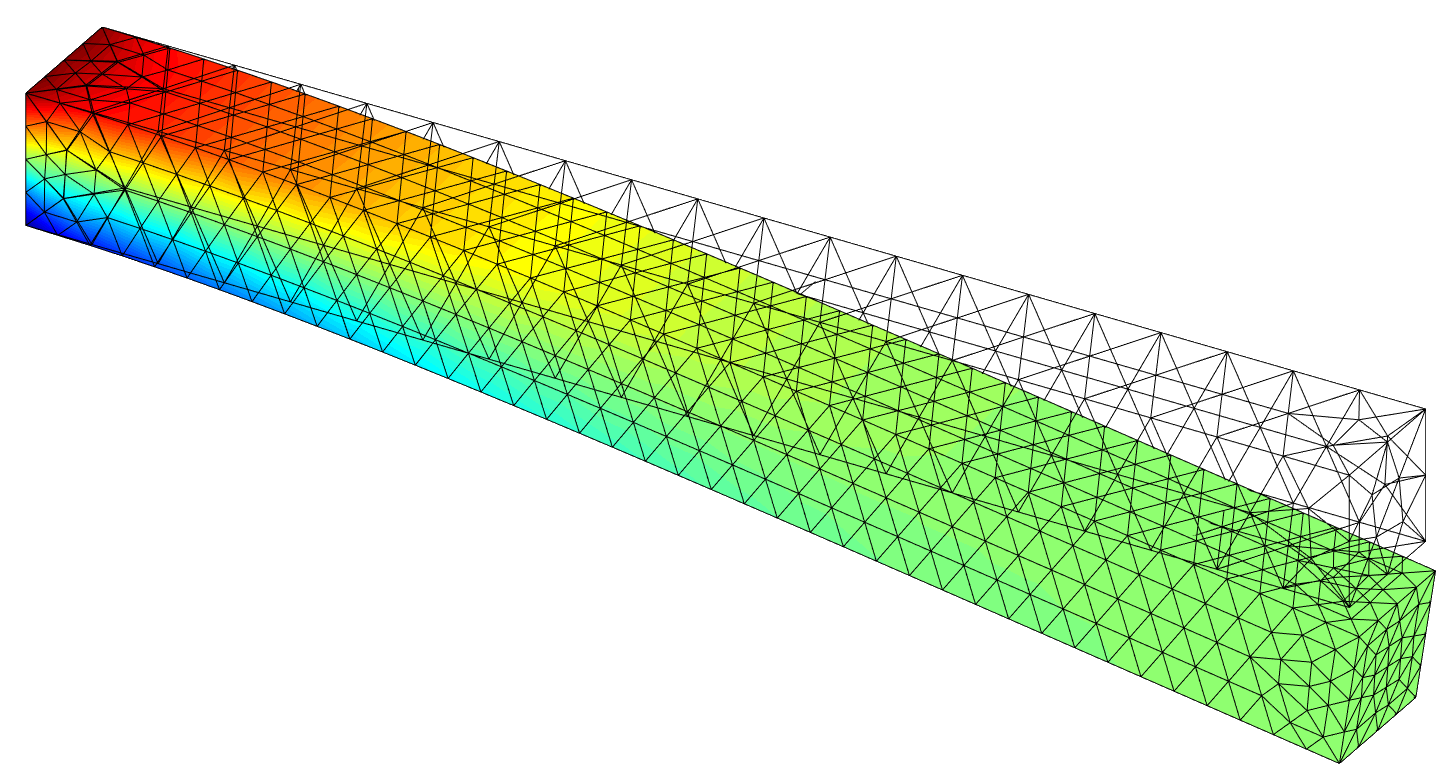
\includegraphics[width=\linewidth]{figure/interpolation.png}
        \caption{Interpolazione mesh bidimensionale.}
    \end{figure}

    \subsection{Gradi di libertà}\label{dof}
    I gradi di libertà rappresentano il numero di componenti, in termini di variabili, da identificare per determinare completamente la soluzione di un problema. Ogni nodo della mesh con cui si sta lavorando
    può avere uno o più gradi di libertà. Per esempio il nodo di una mesh che modella un fluido può avere i seguenti gradi di libertà (componenti che variano):
    \begin{itemize}
        \item Tre componenti per la traslazione
        \item Pressione
        \item Temperatura
    \end{itemize}
    per un totale di cinque gradi di libertà per nodo. In una mesh con 100 nodi ci troveremo a dover calcolare la variazione di 500 gradi di libertà per ogni time step.
    Essendo parametri che governano lo stato fisico di un sistema possono variare in base alle circostanze, ma in ogni caso queste dimensioni vanno regolate da funzioni altrimenti
    non sarebbe possibile computare soluzioni per esse.
    Nella figura \ref*{fig:meshdof} è possibile notare come per una stessa superfice si possono impostare diversi livelli di risoluzione attraverso l'aumento di nodi e, quindi, gradi di libertà.
    \begin{figure}[H]\label{fig:meshdof}
        \centering
        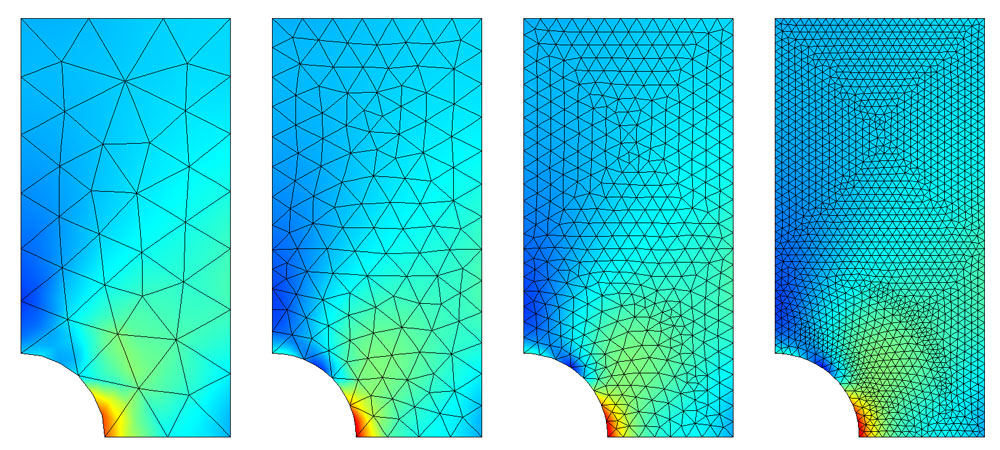
\includegraphics[width=\linewidth]{figure/meshdof.jpg}
        \caption{Differenze di gradi di libertà fra mesh uguali.}
    \end{figure}
    
    \subsection{Metodi Lagrangiani-Euleriani}\label{lagrangian-eulerian}
    Il solver necessità dei metodi numerici e delle particolari istruzioni per interpretare nel modo corretto il problema e trovare una soluzione, in questa sottosezione analizzeremo
    l'approccio utilizzato dal solver implementato durante lo sviluppo di questo progetto.

    Tipicamente i metodi per predirre il movimento di un flusso di particelle si rifanno all'approccio Lagrangiano, particolarmente adatto a tracciare il movimento delle stesse,
    mentre per Flussi (non di particelle) l'approccio Euleriano va per la maggiore.
    L'approccio utilizzato per implementare il solver in questione è un particolare metodo basato su Eulero nel calcolo del flusso del gas presente nell'ugello e su Lagrange
    per quanto riguarda il flusso di particelle metalliche. Si tratta quindi di un approccio ibrido che combina entrambi i metodi per computare più efficacemente la soluzione.
    Analizziamo nel dettaglio in cosa differiscono i due metodi nelle prossime due sottosezioni.
        \subsubsection{Metodo Lagrangiano}
        Il metodo Lagrangiano è caratterizzato poiché si studiano gli elementi in base al cambiamento della loro traiettoria.
        L'approccio Lagrangiano discretizza la massa delle particelle e quindi simula il fluido attraverso il movimento delle particelle stesse del fluido. Maggiore è il numero di particelle
        maggiore sarà la risoluzione della simulazione computata.
        Il metodo Lagrangiano, all'interno di questo progetto, è stato implementato seguendo proprio il concetto di tracciamento di particella; quindi ogni particella all'interno della simulazione
        viene aggiornata in tutte le sue proprietà secondo l'influenza del flusso (calcolato in modo Euleriano) per ogni time step. Nella pratica questo meccanismo si potrebbe tradurre nel
        monitoraggio delle proprietà e della posizione di una singola particella metallica durante tutto il percorso all'interno, e all'esterno prima della posa, dell'ugello.
        \subsubsection{Metodo Euleriano}
        Nel caso del metodo Euleriano è solito trattare direttamente i volumi di fluido fissi nello spazio, studiandone la variazione nello spazio e nel tempo.
        Viene infatti discretizzato lo spazio del dominio introducendo una griglia fissa (\ref{mesh}) i cui nodi vengono definiti con dei valori che descrivono l'evoluzione del fluido nel tempo.
        Questi valori che descrivono i nodi della griglia non sono altro che i gradi di libertà accennati prima (\ref{dof}).
        Uno dei problemi che si pongono utilizzando questo metodo è il modo in cui si fissa la risoluzione della simulazione in base alla griglia, che ricordiamo essere fissa. In parte si può ovviare
        a questo problema adoperando dei metodi Euleriani adattivi.
        Volendo fornire un esempio pratico anche per questo metodo, possiamo visualizzare la tecnica Euleriana come il monitoraggio delle proprietà del flusso in determinati punti fissi del dominio
        attorno all'ugello.
    \subsection{Ouptut}
    Una volta calcolate le soluzioni ai problemi precedentemente descritti è necessario fornire i risultati in formati comprensibili da programmi di visualizzazione o post processing (\ref*{visualizzazione}).
    Spesso i solutori tendono a produrre gruppi di file, almeno uno per time step, per garantire la visualizzazione dell'evoluzione della simulazione durante il corso del tempo, opportunamente discretizzato.
    Per ottenere la massima flessibilità di visualizzazione e post processing dopo la risoluzione della simulazione è necessario includere quante più informazioni possibili all'interno dei file prodotti.
    In particolare è opportuno salvare ogni valore, di ogni proprietà dei nodi e delle particelle, per ogni time step cosi da rendere possibili avanzate tecniche di analisi di andamenti scalari 
    (semplici grafici valore-tempo) e vettoriali (tracing).

\section{Applicazioni comuni}
Forti di quanto appreso fino a questo punto possiamo analizzare alcune, ma di certo non tutte, applicazioni comuni che tutt'ora sono utilizzate in ambito CFD.
Sicuramente in ambito ingegneristico le tecniche simulative CFD trovano riscontro in molte realtà, tra queste vale la pena citarne alcune:
\begin{itemize}
    \item \textbf{Analisi flussi turbolenti e cavitazioni:} la CFD è alla base dello studio riguardo la riduzione (in casi rari dell'aumento) delle turbolenze indotte da superifici. 
    Basti pensare alla progettazione di autoveicoli da corsa il cui profilo aereodinamico è alla base delle alte prestazioni in situazioni ad alta velocità. Nella progettazione di 
    elementi rotativi immersi in fluidi (eliche marine o non) si cerca di ridurre al minimo turbolenze e cavitazioni.
\begin{figure}[H]
    \centering
    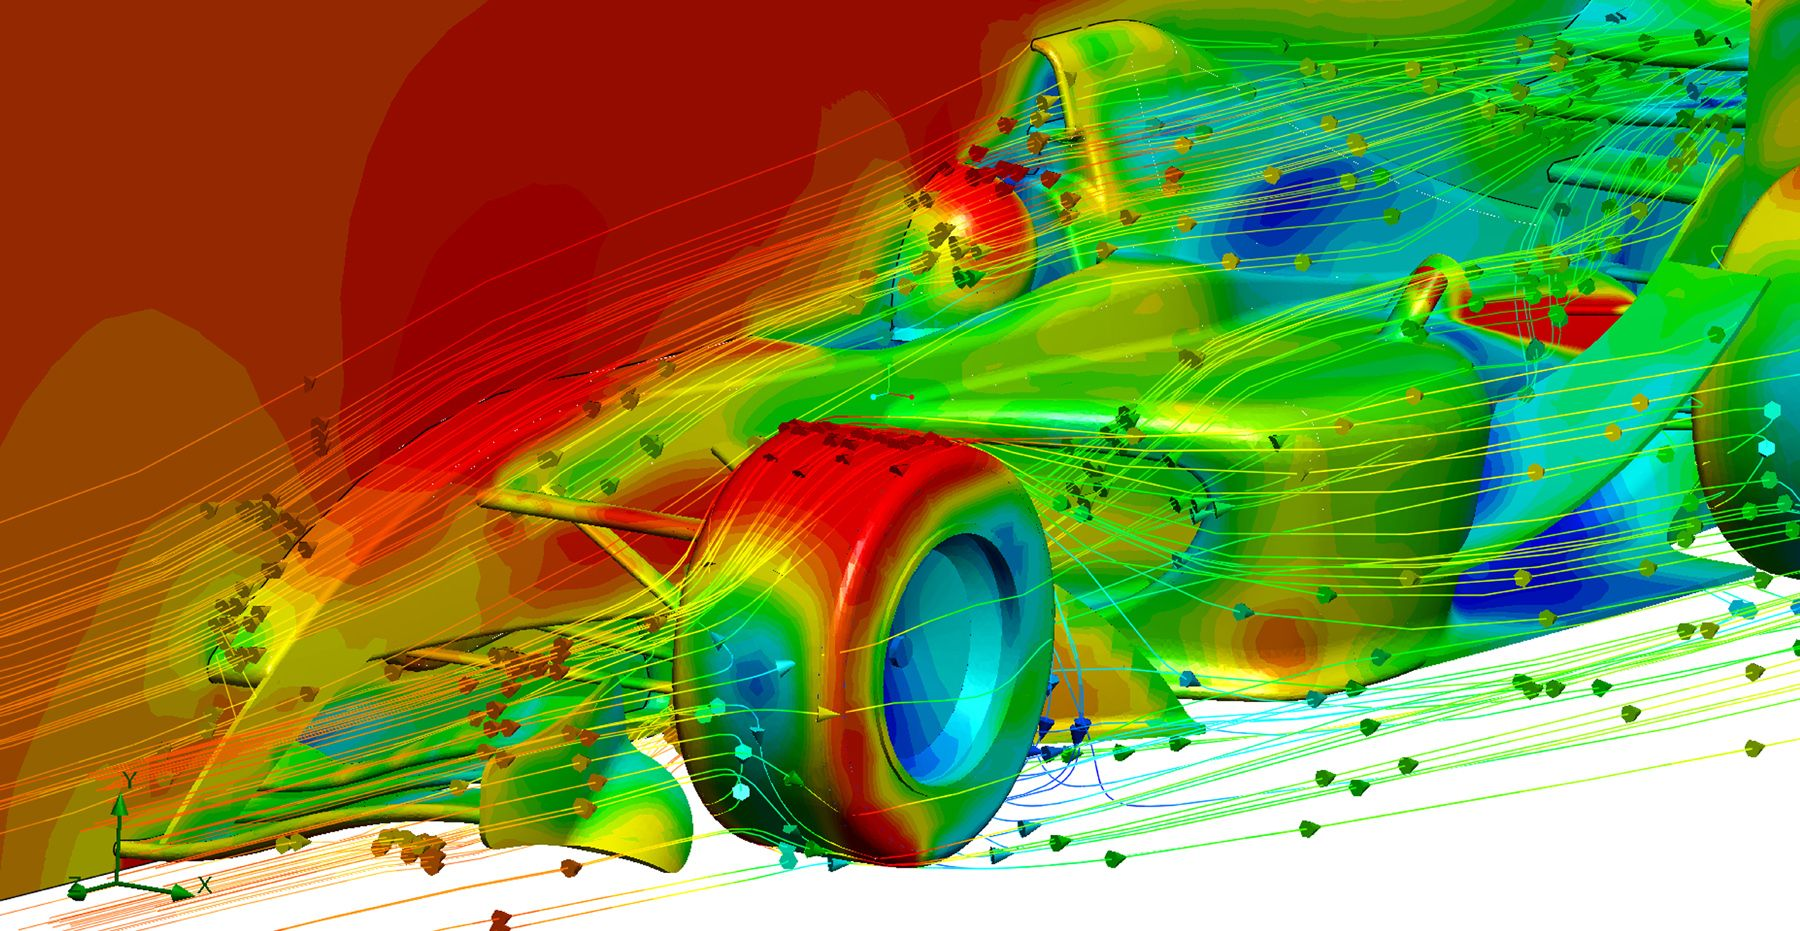
\includegraphics[width=\linewidth]{figure/racecar.jpg}
    \caption{Raffigurazione di una simulazione CFD sul profilo aereodinamico di una macchina da corsa.}
\end{figure}
    \item \textbf{Analisi termica e barometrica di flussi:} in questa categoria ricadono tutte quelle simulazioni atte a predirre il comportamento di fluidi caldi o freddi all'interno di strutture
    solide soggette a espansioni termiche. Un esempio può essere la simulazione di complessi impianti idraulici e di riscaldamento centralizzati.
    \begin{figure}[H]
        \centering
        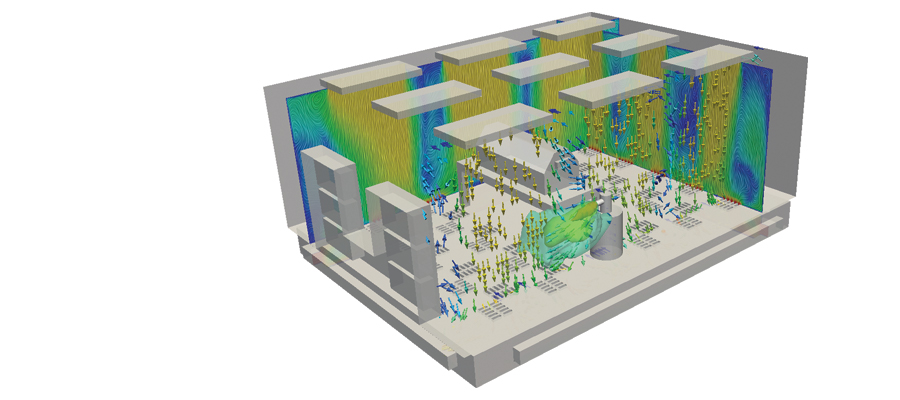
\includegraphics[width=\linewidth]{figure/HVAC-system.jpg}
        \caption{Raffigurazione di una simulazione CFD per un impianto di riscaldamento.}
    \end{figure}
    \item \textbf{Analisi di performance motori a stato solido/liquido per razzi e velivoli:} un analisi dettagliata di come il flusso di un motore a reazione vari in base a determinate proprietà
    del fluido è di vitale importanza nella progettazione dello stesso. La CFD taglia notevolmente i costi di implementazione di nuove tecnologie in quanto è possibile ottenere risultati 
    particolarmente precisi senza dover affrontare l'intero processo produttivo, ma utilizzando esclusivamente risultati numerici propriamente verificati.
    \begin{figure}[H]
        \centering
        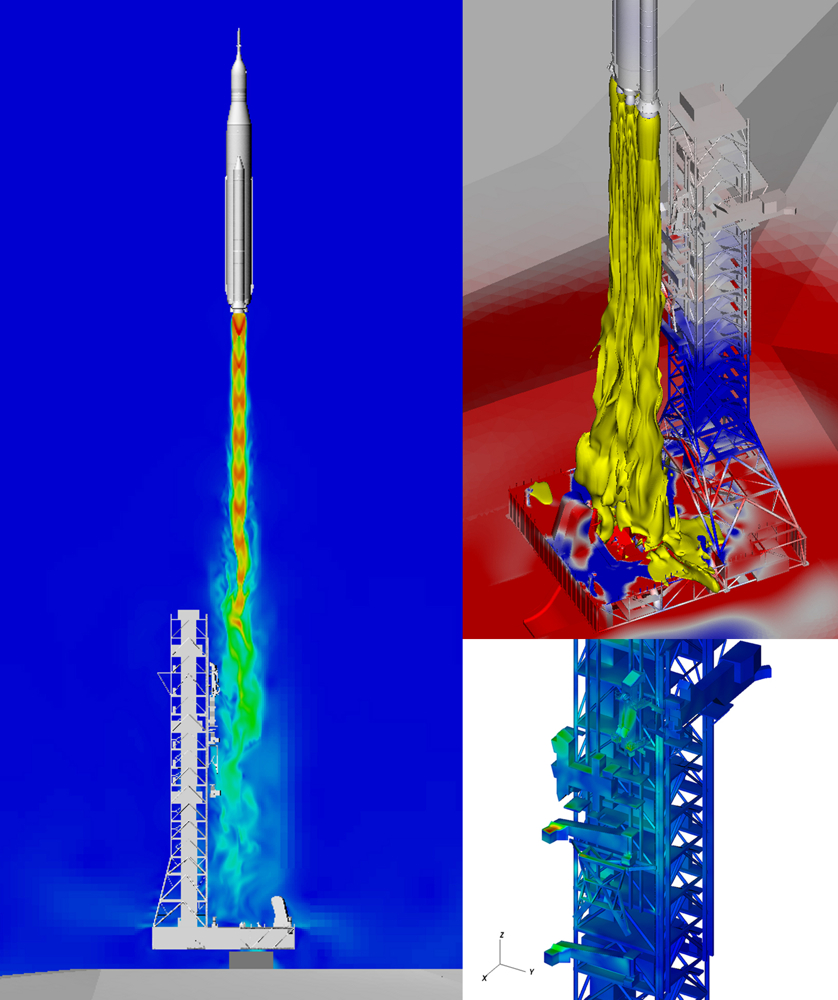
\includegraphics[width=\linewidth]{figure/rocket.jpg}
        \caption{Raffigurazione di una simulazione CFD della fase iniziale di lancio di un razzo.}
    \end{figure}
\end{itemize}
La CFD, da qualche anno a questa parte, ha fatto il suo debutto anche in ambiti d'intrattenimento. Le basi della CFD infatti sono state adattate a problemi relativamente più semplici, 
che non richiedono una soluzione numericamente precisa, bensì più mirata a produrre simulazioni visivamente convincenti.
Questi ambiti riguardano principalmente l'industria cinematografica e videoludica. Queste ultime in particolare stanno spingendo molto la ricerca di soluzioni CFD estremamente veloci e parallelizzabili 
su schede video per simulare al meglio effetti visivi convincenti. 
\begin{figure}[H]
    \centering
    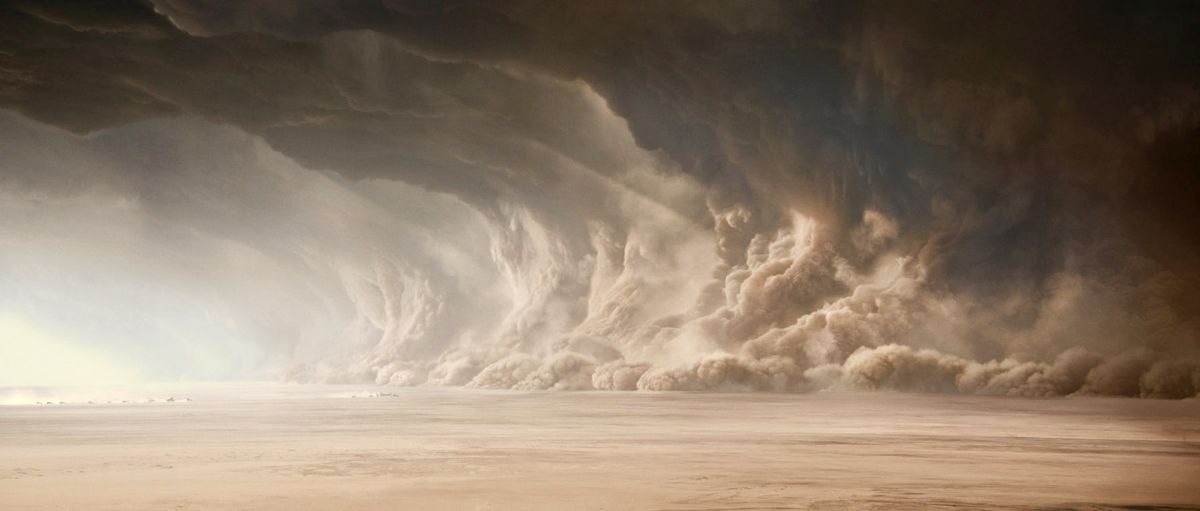
\includegraphics[width=\linewidth]{figure/madmax.jpg}
    \caption{Tempesta di sabbia simulata con tecniche CFD, scena tratta dal film 'Mad Max: Fury Road'.}
\end{figure}
\begin{figure}[H]
    \centering
    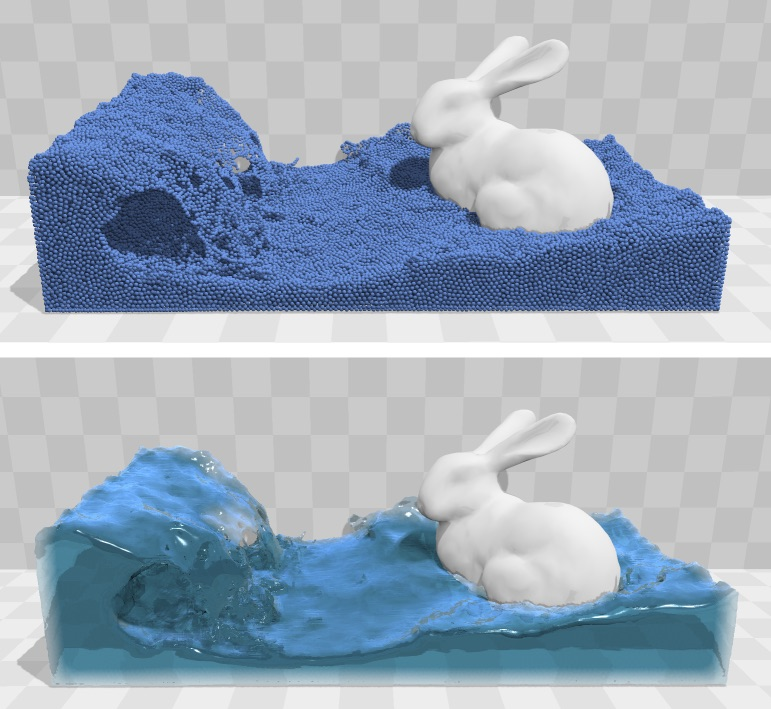
\includegraphics[width=\linewidth]{figure/pbf.jpeg}
    \caption{Simulazione di fluidi in tempo reale, oggetto dell'articolo \cite{macklin2013position}.}
\end{figure}